\subsection{General Concepts}
\label{sec:deep_basics}

The basic building blocks of an \ac{ANN} are Artificial Neurons, which are inspired by  their biological counterparts.
Biological neurons receive a signal via dendrites and output the processed signal through the axon \cite{bioneuron}.
TODO How the signal is processed depends on the biological structure of the neuron.
In general a biological neuron produces an output signal, when a certain activation potential is reached.

The first artificial neuron was proposed in 1958 by Rosenblatt \cite{perceptron} and is known as the Rosenblatt Perceptron.
The decision rule for the Perceptron is described by eq. \ref{form:perceptron}.
It states that the output $\hat{y} \in \{-1, 1\}$ is defined by the sign of the dot product of a weight vector $V \in \R^{n \times 1}$ with an input vector $x \in \R^{n \times 1}$.
The decision boundary of this function is a linear function, which means non-linear problems like the XOR-problem, can't be solved with the perceptron TODO CITE.

\begin{equation}
    \hat{y} = sign(V^Tx)
    \label{form:perceptron}
\end{equation}

To tackle this insufficiency the \ac{MLP} was introduced \cite{mlp}, which is able to solve non-linear problems.
The \ac{MLP} is created by using the output of multiple perceptrons as an input to another perceptron.
In fig. \ref{fig:mlp} the general structure of a \ac{MLP} is shown.
This particular \ac{MLP} has two neurons in the first layer and one in the second layer.
In general the number for neurons inside a layer, as the number of layers is not bounded.

\subsubsection{Learning Procedure}
The learning procedure of an \ac{ANN} is as follows:

\begin{enumerate}
    \item The input data gets fed into the network and produces an output.
    \item The similarity of the output and the desired output (label) are measured using a loss function.
    \item The loss is used to calculate the gradients by propagating it back through the network TODO chainrule.
    \item The gradients are used in a gradient descent algorithm to update and optimize the weights of the network.
    \item The above is performed until the weights don't change anymore.
\end{enumerate}

\subsubsection{Forward Propagation}
As with the perceptron the input vector $x$ gets multiplied with the corresponding weights $W_{n,i}$, where $n$ denotes the index of the neuron in the layer and $i$ the index of the input vector $x$.
After the multiplication the results are summed up and are forwarded to an activation function.
The results of the activation function are now inputs for the second layer and the above is repeated.
In the end, the second layer activation function produces an output $\hat{y}$.

\subsubsection{Loss}
After the output $\hat{y}$ was calculated a loss function is applied to $\hat{y}$ and the  label $y$.
The most prominent of these loss functions is the \ac{MSE} (see eq. \ref{eq:mse}).
The \ac{MSE} takes the labels and the output and calculates the sum of the differences between the two vectors.
Finally, the mean is taken of the resulting sum, where $n$ here denotes the dimensionality of $y$ and $\hat{y}$.

\begin{equation}
    \label{eq:mse}
    MSE(y, \hat{y}) = \frac{1}{n} \sum_{i=1}^{n}(y_i - \hat{y}_i)^2
\end{equation}

\subsubsection{Backward Propagation}

To make an \ac{ANN} learn the

While in the perceptron the sign function is used as an activation function, for \acp{MLP} this is not a good choice, because the sign function is non-differentiable.
In particular, this is important because a gradient is needed to update the weights of an \ac{MLP} during training.

\begin{figure}[t]
	\centering
	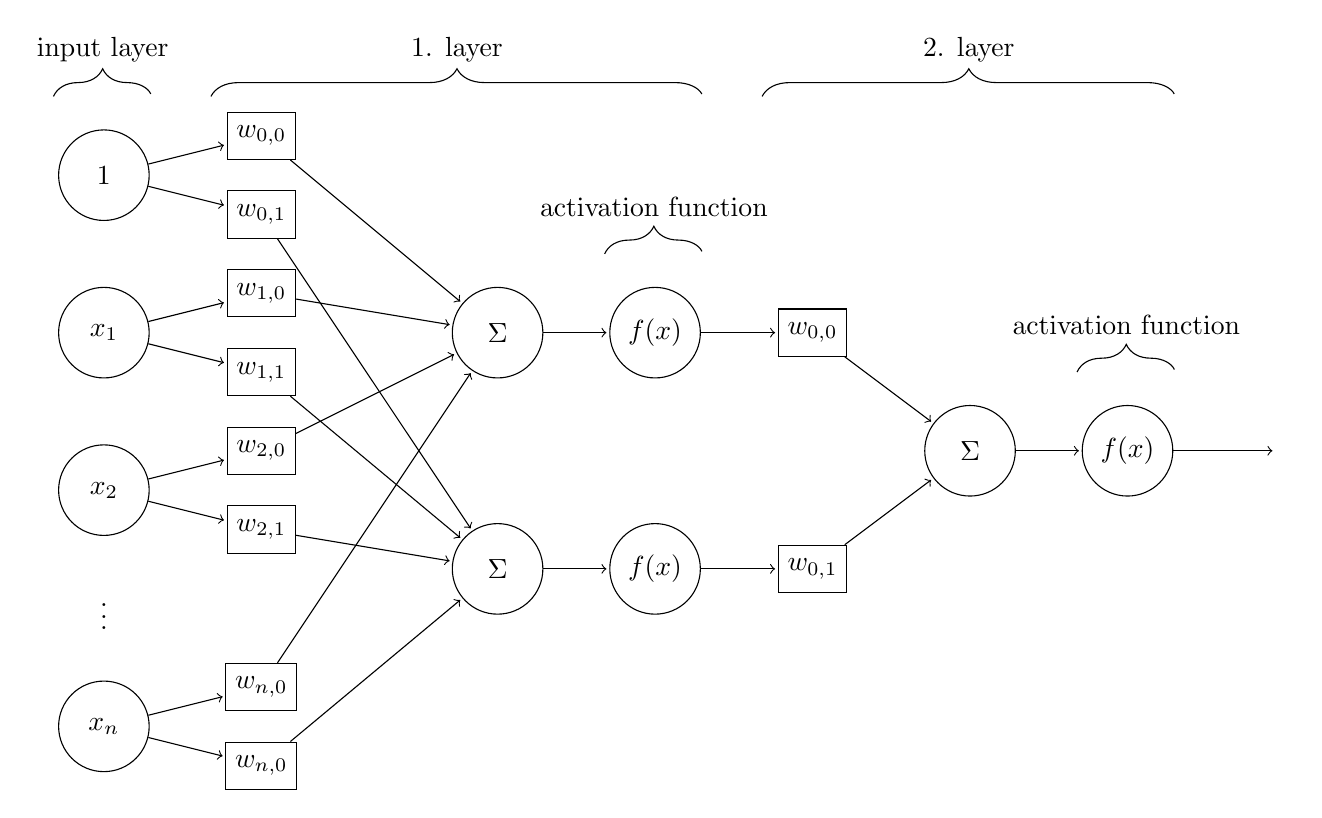
\begin{tikzpicture}[shorten >=1pt]
		\tikzstyle{unit}=[draw,shape=circle,minimum size=1.15cm]
		\tikzstyle{hidden}=[draw=none]
        \tikzstyle{weight}=[draw,shape=rectangle,minimum size=0.6cm]


        % input layer
        \node[unit](b0) at (0, 7, 0){$1$};
        \node[unit](x1) at (0, 5, 0){$x_1$};
        \node[unit](x2) at (0, 3, 0){$x_2$};
        \node at (0, 1.5){\vdots};
        \node[unit](xn) at (0, 0, 0){$x_n$};
		\draw [decorate,decoration={brace,amplitude=10pt},xshift=-4pt,yshift=0pt] (-0.5,8) -- (0.75,8) node [black,midway,yshift=+0.6cm]{input layer};

        % weight layer
        \node[weight](w00) at (2, 7.5, 0){$w_{0,0}$};
        \node[weight](w01) at (2, 6.5, 0){$w_{0,1}$};

        \node[weight](w10) at (2, 5.5, 0){$w_{1,0}$};
        \node[weight](w11) at (2, 4.5, 0){$w_{1,1}$};

        \node[weight](w20) at (2, 3.5, 0){$w_{2,0}$};
        \node[weight](w21) at (2, 2.5, 0){$w_{2,1}$};

        \node[weight](wn0) at (2, 0.5, 0){$w_{n,0}$};
        \node[weight](wn1) at (2, -0.5, 0){$w_{n,0}$};

        % sum layer
        \node[unit](sum0) at (5, 5, 0){$\Sigma$};
        \node[unit](sum1) at (5, 2, 0){$\Sigma$};

        % activation layer
        \node[unit](acti0) at (7, 5, 0){$f(x)$};
        \node[unit](acti1) at (7, 2, 0){$f(x)$};
		\draw [decorate,decoration={brace,amplitude=10pt},xshift=-4pt,yshift=0pt] (6.5,6) -- (7.75,6) node [black,midway,yshift=+0.6cm]{activation function};

		\draw [decorate,decoration={brace,amplitude=10pt},xshift=-4pt,yshift=0pt] (1.5,8) -- (7.75,8) node [black,midway,yshift=+0.6cm]{1. layer};

        % weight layer 2
        \node[weight](w200) at (9, 5, 0){$w_{0,0}$};
        \node[weight](w201) at (9, 2, 0){$w_{0,1}$};

        % sum layer 2
        \node[unit](sum2) at (11, 3.5, 0){$\Sigma$};

        % activation layer 2
        \node[unit](acti2) at (13, 3.5, 0){$f(x)$};
		\draw [decorate,decoration={brace,amplitude=10pt},xshift=-4pt,yshift=0pt] (12.5,4.5) -- (13.75,4.5) node [black,midway,yshift=+0.6cm]{activation function};


		\draw [decorate,decoration={brace,amplitude=10pt},xshift=-4pt,yshift=0pt] (8.5,8) -- (13.75,8) node [black,midway,yshift=+0.6cm]{2. layer};

        % hidden output
        \node[hidden](h0) at (15, 3.5, 0){};

        \draw[->](b0) -- (w00);
        \draw[->](b0) -- (w01);

        \draw[->](x1) -- (w10);
        \draw[->](x1) -- (w11);

        \draw[->](x2) -- (w20);
        \draw[->](x2) -- (w21);

        \draw[->](xn) -- (wn0);
        \draw[->](xn) -- (wn1);

        \draw[->](w00) -- (sum0);
        \draw[->](w10) -- (sum0);
        \draw[->](w20) -- (sum0);
        \draw[->](wn0) -- (sum0);

        \draw[->](w01) -- (sum1);
        \draw[->](w11) -- (sum1);
        \draw[->](w21) -- (sum1);
        \draw[->](wn1) -- (sum1);

        \draw[->](sum0) -- (acti0);
        \draw[->](sum1) -- (acti1);

        \draw[->](acti0) -- (w200);
        \draw[->](acti1) -- (w201);

        \draw[->](w200) -- (sum2);
        \draw[->](w201) -- (sum2);

        \draw[->](sum2) -- (acti2);
        \draw[->](acti2) -- (h0);

	\end{tikzpicture}
	\caption{Multi Layer Perceptron with two layers}
	\label{fig:mlp}
\end{figure}


\subsubsection{Optimization}

\subsection{Convolutional Neural Networks}

While \acp{MLP} perform pretty well on vectorial data, multidimensional data like images for example, can only be fed to a network when it was previously flattened into a vector.
One problem that arises is that when flattening for example an image of size $100 \times 100$, this would already require the input size of the network to have $10.000$ weights per neuron in the next layer.
This increases drastically the capacity of the network and hence requires a larger training set.
Additionally nearby pixels in images are often highly correlated and classical unstructured \ac{ANN} fails to capture such spatial dependencies. \cite{lecun_lenet}

- TODO transforms and bla

The proposed alternative therefor are \acp{CNN}, which have shown to perform pretty well over the last decade in several image related benchmarks. \cite{inception}, \cite{resnet}, \cite{densenet}.
The classical \ac{CNN} architecture is comprised of three different layer types:

\begin{itemize}
    \item convolutional layers
    \item pooling layers
    \item fully-connected layers
\end{itemize}

\subsubsection{Convolutional Layer}
Convolutional layers form the major component in a \ac{CNN}.
As the name suggest the underlying mathematical foundation of those layers is the convolution.
The equation for a convolution (see eq. \ref{eq:conv}), states that a function $f$ convolved with another function $g$, is the multiplication of those two functions, while $g$ is shifted over $f$.
The final result is then obtained by taking the integral over the whole domain. \cite{dl}

\begin{equation}
    (f * g)(x) = \int_{-\infty}^{\infty}f(\tau)g(x - \tau)d\tau
    \label{eq:conv}
\end{equation}

In simpler terms that just means there is an image $I \in \R^{WxHxC}$, where $W$ and $H$ are the width and height of the image and $C$ being the number of channels.
Furthermore, there is a kernel $K$ with $K \in \R^{W_KxH_KxC}$.
The image and the kernel are now convolved by moving the kernel over the image and at each position an element-wise multiplication of the overlapping area of the image and the kernel is taken.
Afterwards, the result is summed up and used as an output element in the convolution result.
Finally, the kernel is shifted further until the whole image has been convolved.
How much pixel a kernel is shifted at a time depends on the used stride.
The higher the stride the less local information is preserved.
Typically a stride of $1$ or $2$ is used.
An example of a convolution of a $4\times4$ input with a $3\times3$ kernel and a stride of $1$ is given in figure \ref{fig:conv_example}.

\begin{figure}
\begin{center}
    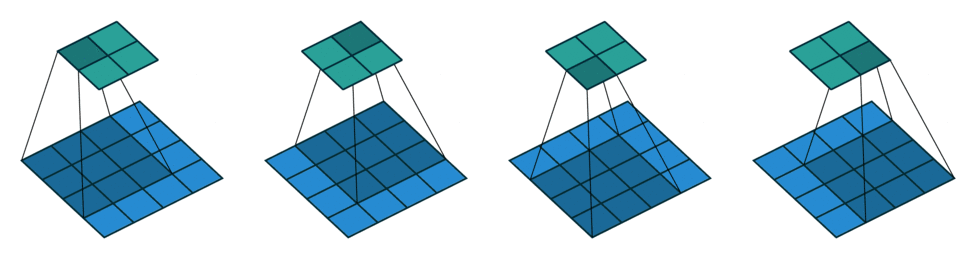
\includegraphics[width=16cm]{imgs/conv_example_full.png}
    \caption{Example convolution of a 4x4 input (blue) with a 3x3 kernel (dark blue) and a stride of 1, resulting in a 2x2 output (cyan) \cite{conv_arithmetic}}
    \label{fig:conv_example}
\end{center}
\end{figure}

- TODO size of output?

- TODO padding?

\subsubsection{Pooling Layer}
Pooling layers in \acp{CNN} are used to further reduce the dimensionality of the output.
During the pooling operation information across spatial locations is fused by sliding a window (typically of size $2\times2$ or $3\times3$) over the input and performing a function on the values inside the window.
In the case of max pooling the used function is the $MAX$ function, therefore only the maximum value inside the window is considered and used in the pooling output.
This decreases the number of parameters and hence reduces the computational cost. \cite{dl}

- TODO average pooling?

- TODO global average?

- TODO maybe Vincents learnable pooling

\subsubsection{Fully-Connected Layer}
The fully-connected layer as described in \ref{sec:deep_basics} is the final layer inside a \ac{CNN}.
Before the calculations of this layer are applied, the input tensor is flattened into a vector.
The input corresponds to some high level features which were previously build through the convolutional and pooling layers.
The last operation in this output layer in a multi-class classification task is normally a softmax activation function \cite{softmax}, which produces a probability vector.
Each element in the vector corresponds to the probability of a class in the task.
The softmax function is defined as:

\begin{equation}
    softmax(x)_i = \frac{e^{x_i}}{\sum_{j=1}^Ne^{x_j}}
\end{equation}

Which basically means that the output probability $softmax(x)_i$ is defined as the fraction of the exponential function applied to an element of the vector, divided by the sum of all exponential function outputs applied to all elements of the vector.

\subsection{Activation Functions}

\subsubsection{Sigmoid}

\subsubsection{Hard Sigmoid}

\subsubsection{Rectified Linear Unit (ReLU)}

\subsubsection{ReLU6}

\subsubsection{Hard Swish}

\subsection{Loss Functions}

- TODO CE

\subsubsection{Skip Connections}

\subsection{Batch Normalization}

\subsection{Dropout}
